% Initial version by Darian Muresan, Ph.D.
% dmuresan@stevens.edu
% Edit and adjust as needed.
\documentclass[12pt]{cornell}

% add index support
%\usepackage{imakeidx}
\usepackage{makeidx}
%\makeindex

% graphing programs
\usepackage{color}
\usepackage{psfrag}
\usepackage{verbatim}
\usepackage{fancyhdr}
%\usepackage{titlesec}
\usepackage{fancyvrb} 
% hyperlink programs
%\usepackage{url}

% Does not work with LaTeX=>PDF
\usepackage[pdfmark, 
breaklinks=true, 
colorlinks=true,
citecolor=blue,
linkcolor=blue,
menucolor=black,
pagecolor=black,
urlcolor=blue
]{hyperref} % links in pdf

%\usepackage[colorlinks]{hyperref} % links in dvi
\usepackage{listings}
\usepackage{amsfonts} 
\usepackage{amssymb} 
%\usepackage{tabto}

\usepackage{tabularx,colortbl}
\usepackage[chapter]{algorithm} 
\usepackage{algorithmic} 
\usepackage{blindtext}

\definecolor{DarkGreen}{rgb}{0,0.6,0}
\definecolor{mygreen}{rgb}{0,0.6,0}
\definecolor{mygray}{rgb}{0.5,0.5,0.5}
\definecolor{mymauve}{rgb}{0.58,0,0.82}

\usepackage{tocloft}
\usepackage{amsmath}
\usepackage{tcolorbox}
\usepackage{enumitem}
\usepackage{longtable}
%\usepackage{textcomp}
\usepackage{txfonts}
\usepackage{pstool}

%part for \part titles
%chap for \chapter titles
%sec for \section titles
%subsec for \subsection titles
%subsubsec for \subsubsection titles
%para for \paragraph titles
%subpara for \subparagraph titles
%fig for figure \caption titles
%subfig for subfigure \caption titles
%tab for table \caption titles
%subtab for subtable \caption titles


% update chapter number spacing
\setlength{\cftchapnumwidth}{2em}
\setlength{\cftsecnumwidth}{2.5em}
\setlength{\cftsubsecnumwidth}{3.5em}
\setlength{\cftsubsubsecnumwidth}{4.5em}

\addtolength{\cftsecindent}{0.5em}
\addtolength{\cftsubsecindent}{0.5em}
\addtolength{\cftsubsubsecindent}{0.5em}

%\titlespacing*{\chapter}{0pt}{-50pt}{20pt}
%\titleformat{\chapter}[display]{\normalfont\huge\bfseries}{\chaptertitlename\ 
%\thechapter}{20pt}{\Huge}
%\pagestyle{fancy}
%\pagestyle{cornell}
%
%\rhead{F054-021-0172}
%\chead{Nonlinear Enhancement of Visual Target Detection (AF05-T021)}
%\lhead{GSTI}
%\lfoot{\scriptsize Use or disclosure of data on this page is subject
%to the restriction on the title page of this proposal.}
%\cfoot{}
%\rfoot{\thepage}

\newfont{\Bp}{msbm10}
\newfont{\BpBig}{msbm10 scaled\magstep2}
\newfont{\Sc}{eusm10}
\newfont{\ScBig}{eusm10 scaled\magstep3}
\newfont{\Fr}{eufm10}
\newfont{\FrBig}{eufm10 scaled\magstep1}

% some commands:
\newcommand{\dxi}{{\tt m\_xDeltaInput}}
\newcommand{\dyi}{{\tt m\_yDeltaInput}}
\newcommand{\dci}{{\tt m\_cDeltaInput}}
\newcommand{\dxo}{{\tt m\_xDeltaOutput}}
\newcommand{\dyo}{{\tt m\_yDeltaOutput}}
\newcommand{\dco}{{\tt m\_cDeltaOutput}}
\newcommand{\ttf}[1]{{\tt #1}}
\newcommand{\tbl}[2]{{\begin{tabular}{c} #1 \\ #2 \end{tabular}}}

\newcommand{\urltwo}[2]{\mbox{\href{#1}{\tt #2}}}
\newcommand{\qnorm}[1]{\|#1\|_{\bQ}}
\newcommand{\qdot}[2]{\lrb #1, #2 \rrb_{\bQ}}
\newcommand{\kdot}[2]{\lrb #1, #2 \rrb_{\bf k}}
\newcommand{\tdot}[2]{\lrb #1, #2 \rrb}
\newcommand{\mydiff}[2]{\lrb #1 - #2 \rrb}
\newcommand{\lena}{\textit{lena}}
\newcommand{\barb}{\textit{barbara}}
\newcommand{\boat}{\textit{boat}}
\newcommand{\leaves}{\textit{leaves}}
\newcommand{\rings}{\textit{rings}}
\newcommand{\treg}{\textit{train region}}
\newcommand{\dreg}{\textit{denoise region}}
\newcommand{\oreg}{\textit{overlap region}}
\newcommand{\sil}{\sigma_l^2}
\newcommand{\sn}{\sigma^2}
\newcommand{\bn}{{\mbox{\bf \FrBig N}}}
\newcommand{\n}{\mbox{\Fr N}}
%\newcommand{\bn}{\bf N}
%\newcommand{\n}{N}
\newcommand{\bY}{\textbf{Y}}
\newcommand{\bX}{\textbf{X}}
\newcommand{\bb}{\textbf{b}}
\newcommand{\bu}{\textbf{u}}
\newcommand{\bv}{\textbf{v}}
\newcommand{\by}{\textbf{y}}
\newcommand{\bx}{\textbf{x}}
\newcommand{\be}{\textbf{e}}
\newcommand{\bz}{\textbf{z}}
\newcommand{\bs}{\textbf{s}}
\newcommand{\bw}{\textbf{w}}
\newcommand{\bQ}{\textbf{Q}}
\newcommand{\bphi}{\textbf{$\phi$}}
\newcommand{\lsb}{\left[}
\newcommand{\rsb}{\right]}
\newcommand{\lrb}{\left(}
\newcommand{\rrb}{\right)}
\newcommand{\lcb}{\left\{}
\newcommand{\rcb}{\right\}}
\newcommand{\R}{\mbox{\BpBig R}}
\newcommand{\F}{{\cal F}}
\newcommand{\Fk}{\mbox{\Sc F}}
\newcommand{\bQF}{\textbf{Q}_{\mbox{\Sc F}}}
\newcommand{\N}{{\cal N}}
\newcommand{\xlz}{X_l(z)}
\newcommand{\xhz}{X_h(z)}
\newcommand{\xz}{X(z)}
\newcommand{\pr}{ perfect reconstruction }
\newcommand{\smb}{Smith-Barnwell }
\newcommand{\xw}{X(e^{j\omega})}
\newcommand{\xmw}{X(-e^{j\omega})}
\newcommand{\dw}{D(e^{j\omega})}
\newcommand{\dmw}{D(-e^{j\omega})}
\newcommand{\ew}{E(e^{j\omega})}
\newcommand{\emw}{E(-e^{j\omega})}
\newcommand{\fw}{F_0(e^{j\omega})}
\newcommand{\fmw}{F_0(-e^{j\omega})}
\newcommand{\hoz}{H_1(z)}
\newcommand{\hzz}{H_0(z)}
\newcommand{\goz}{G_1(z)}
\newcommand{\gzz}{G_0(z)}
\newcommand{\hzw}{H_{0}(e^{j\omega})}
\newcommand{\hzmw}{H_{0}(-e^{j\omega})}
\newcommand{\hzcw}{H_{0}(e^{-j\omega})}
\newcommand{\how}{H_1(e^{j\omega})}
\newcommand{\homw}{H_1(-e^{j\omega})}
\newcommand{\gzw}{G_0(e^{j\omega})}
\newcommand{\gzmw}{G_0(-e^{j\omega})}
\newcommand{\gow}{G_1(e^{j\omega})}
\newcommand{\gomw}{G_1(-e^{j\omega})}
\newcommand{\wl}{e^{-jwL}}
\newcommand{\aqua}{\textit{AQua with OR }}
\newtheorem{theorem}{Theorem}
\newtheorem{lemma}{Lemma}
\newtheorem{corollary}{Corollary}
\newtheorem{claim}{Claim}
\newtheorem{definition}{Definition}
\newenvironment{proof}{\noindent{\em Proof.}}{\ \hfill Q.E.D.}
%\newtheorem{moduleCount}{L}
\newcommand*{\labelfile}[1]{%
  \label{file:#1}%
}

% Use this to label requirements, use cases, user stories, etc.
% This is where we can add different spellings for different types of 
% requirements, use cases, user stories, etc.
% \newtheorem{requirementKind}{Requirement Spelling}
\newtheorem{reqkFunctional}{Functional Requirement}
\newtheorem{reqkQuality}{Quality Requirement}
\newtheorem{reqkConstraint}{Constraint Requirement}
\newtheorem{reqkInterface}{Interface Requirement}
\newtheorem{reqkBusiness}{Business Requirement}
% Use cases
\newtheorem{useCase}{Use Case}
% User story
\newtheorem{userStory}{User Story}

% command for adding a version to the document
\newcommand{\VERSION}{Version 0.0.0}

% Family -- enter the name of the family that it belongs to: Chapter, Figure, Table, etc.
% Name -- name of the family member: file name, table name, etc.
\newcommand{\FamilyName}[2]{\hyperref[#1::#2]{#2}\index{#2}\xspace}
% Family -- same as above
% Name -- same as above
% Reference -- shorthand for the 'Name'.  It will show as Reference_NameID
% Kind -- underscore(_), space, or dash (-)
\newcommand{\FamilyNameReferenceKind}[4]{\hyperref[#1::#2]{$#3#4{\ref*{#1::#2}}$}}
% newcommand{Family,Label}
\newcommand{\FamilyLabel}[2]{\label{#1::#2}}


% for use cases
\newcommand{\UseCaseLabel}[1]{\FamilyLabel{UseCase}{#1}}
\newcommand{\UseCaseName}[1]{\FamilyName{UseCase}{#1}}
\newcommand{\UseCaseReference}[1]{\FamilyNameReferenceKind{UseCase}{#1}{UC}{_}}
% UseCase name with stacked reference
\newcommand{\UseCaseNameWSReference}[1]{\begin{tabular}{c}\UseCaseName{#1} \\ (\UseCaseReference{#1}) \end{tabular}}
% UseCase name with inline reference
\newcommand{\UseCaseNameWIReference}[1]{\UseCaseName{#1} (\UseCaseReference{#1})}

% for chapters
\newcommand{\ChapterName}[1]{\FamilyName{Chapter}{#1}}
\newcommand{\ChapterLabel}[1]{\FamilyLabel{Chapter}{#1}}
\newcommand{\ChapterReference}[1]{\FamilyNameReferenceKind{Chapter}{#1}{Chapter}{\mbox{ }}}
% Chapter name with inline (WI) reference 
\newcommand{\ChapterNameWIReference}[1]{\ChapterName{#1} (\ChapterReference{#1})}

% for figures
\newcommand{\FigureName}[1]{\FamilyName{Figure}{#1}}
\newcommand{\FigureLabel}[1]{\FamilyLabel{Figure}{#1}}
\newcommand{\FigureReference}[1]{\FamilyNameReferenceKind{Figure}{#1}{Figure}{\mbox{ }}}
% Figure name with stacked (WS) reference
\newcommand{\FigureNameWSReference}[1]{\begin{tabular}{c}\FigureName{#1} \\ (\FigureReference{#1}) \end{tabular}}
% Figure name with inline (WI) reference 
\newcommand{\FigureNameWIReference}[1]{\FigureName{#1} (\FigureReference{#1})}

% for tables
\newcommand{\TableName}[1]{\FamilyName{Table}{#1}}
\newcommand{\TableLabel}[1]{\FamilyLabel{Table}{#1}}
\newcommand{\TableReference}[1]{\FamilyNameReferenceKind{Table}{#1}{Table}{\mbox{ }}}

% for requirements
% RequirementLabel[Kind][Label]
\newcommand{\RequirementLabel}[2]{\FamilyLabel{#1}{#2}}
\newcommand{\RequirementName}[2]{\FamilyName{#1}{#2}}
\newcommand{\RequirementReference}[2]{\FamilyNameReferenceKind{#1}{#2}{#1}{_}}
% Requirements name with stacked (WS) reference
\newcommand{\RequirementNameWSReference}[2]{\begin{tabular}{c}\RequirementName{#1}{#2} \\ (\RequirementReference{#1}{#2}) \end{tabular}}
% Requirements name with inline (WI) reference 
\newcommand{\RequirementNameWIReference}[2]{\RequirementName{#1}{#1} (\RequirementReference{#1}{#2})}

% for requirements
% RequirementLabel[Kind][Label]
\newcommand{\UserStoryLabel}[2]{\FamilyLabel{#1}{#2}}
\newcommand{\UserStoryName}[2]{\FamilyName{#1}{#2}}
\newcommand{\UserStoryReference}[2]{\FamilyNameReferenceKind{#1}{#2}{R}{_}}
% Requirements name with stacked (WS) reference
\newcommand{\UserStoryNameWSReference}[2]{\begin{tabular}{c}\RequirementName{#1}{#2} \\ (\RequirementReference{#1}{#2}) \end{tabular}}
% Requirements name with inline (WI) reference 
\newcommand{\UserStoryNameWIReference}[2]{\RequirementName{#1}{#1} (\RequirementReference{#1}{#2})}



\lstset{ %
  backgroundcolor=\color{white},   % choose the background color; you must add \usepackage{color} or \usepackage{xcolor}
  basicstyle=\footnotesize,        % the size of the fonts that are used for the code
  breakatwhitespace=false,         % sets if automatic breaks should only happen at whitespace
  breaklines=true,                 % sets automatic line breaking
  captionpos=b,                    % sets the caption-position to bottom
  commentstyle=\color{DarkGreen},    % comment style
  deletekeywords={...},            % if you want to delete keywords from the given language
  escapeinside={\%*}{*)},          % if you want to add LaTeX within your code
  extendedchars=true,              % lets you use non-ASCII characters; for 8-bits encodings only, does not work with UTF-8
  %frame=single,                   % adds a frame around the code
  keepspaces=true,                 % keeps spaces in text, useful for keeping indentation of code (possibly needs columns=flexible)
  keywordstyle=\color{blue},       % keyword style
  language=C++,                    % the language of the code
  morekeywords={*,...},            % if you want to add more keywords to the set
  numbers=left,                    % where to put the line-numbers; possible values are (none, left, right)
  numbersep=5pt,                   % how far the line-numbers are from the code
  numberstyle=\tiny\color{mygray}, % the style that is used for the line-numbers
  rulecolor=\color{black},         % if not set, the frame-color may be changed on line-breaks within not-black text (e.g. comments (green here))
  showspaces=false,                % show spaces everywhere adding particular underscores; it overrides 'showstringspaces'
  showstringspaces=false,          % underline spaces within strings only
  showtabs=false,                  % show tabs within strings adding particular underscores
  stepnumber=1,                    % the step between two line-numbers. If it's 1, each line will be numbered
  stringstyle=\color{mymauve}     % string literal style
  %tabsize=2,                      % sets default tabsize to 2 spaces
  %caption=\lstname                % show the filename of files included with \lstinputlisting; also try caption instead of title
}


% Uncomment draftcopy to get the word DRAFT boldly across the first page
%   By the way, xdvi won't show it but it will come out when you print
%\usepackage[light,all]{draftcopy}		% DRAFT on first page
%\draftcopySetGrey{.97}
%\draftcopyName{Confidential}{150}
%\draftcopFirstPage{1}

% Uncomment drafthead to get the date and DRAFT in the header of pages
% that are normallly numbered on the top, pages 2-n of each chapter for example
% This doesn't work with centered page numbers: \pagestyle{cornellc}
%\usepackage{drafthead}

% glossaries to organize the document glossary
%\usepackage[toc,chapter,numberedchapter = autolabel]{glossaries}
\usepackage{glossaries}
\usepackage{minted}

% glossary creation
\newglossaryentry{must}
{	name={MustHave},
	description={This defines the first highest priority requirement.
	All of the tasks, requirements, or anything that is marked this way are
	build in the current version}
}

\newglossaryentry{should}
{	name={ShouldHave},
	description={This defines the second highest priority requirement. The system should implement 
	all of the tasks, requirements, or anything that is marked this way, but if 
	resources are limited, it can be left out of the current version.
	Build in next version}
}

\newglossaryentry{could}
{	name={CouldHave},
	description={This defines the third highest priority requirement.The system could implement 
	all of the tasks, requirements, or anything that is marked this way, but if 
	resources are limited, it can be left out of the current and next version.
	Build in two versions from now}
}

\newglossaryentry{would}
{	name={WouldHave},
	description={This defines the lowest priority requirement.  The system would like to implement 
all of the tasks, requirements, or anything that is marked this way, but only
if resources are available. It can be left out of all future versions}
}

\newglossaryentry{cicd}{
    name={CI/CD},
    description={Continuous Integration and Continuous Deployment - automated software development practices that enable frequent code integration and deployment}
}
%\makeglossaries
\makenoidxglossaries
\makeindex

% Including selective chapters:
% use this to selectively process chapters, etc.  Put a % in front of
% the sections that you don't want done this time.  Includes are
% used instead of \input so that LaTeX will keep track of chapters and
% pages without processing everything.  Don't let any spaces creep in
% around the words or it will not work!

\includeonly{
prologue,
itIntroduction,
history,
itKanban,
itPasswords,
itHosts,
docker,
projectProposal,
itAppendix
}


\begin{document}

\pagenumbering{roman}
\singlespacing
% File: prologue.tex
% Thesis prologue:  Title page, acknowledgements, table of contents,
% list of figures, and list of tables.
%
% this file is to be \include'd after the \begin{document}

% Cornell-style title page
\begin{titlepage}
        \title{DevOps Fall 2025 Overleaf}
        \author{Andre Santiago Neyra, Badri Narayanan R \\ Stevens.edu }
        \conferraldate{}{\today} \maketitle
\end{titlepage}

% Copyright page
%\begin{copyrightpage}
\makecopyright
%\end{copyrightpage}

% Abstract: the abstract body is pulled from the file abstract.tex;
%  the title is pulled from the \title command in the titlepage section
\begin{abstract}
        %\makeabstitle
        \input abstract      % puts the abstract file here
\end{abstract}

% Biographical information pulled from file bio.tex
%\begin{biosketch} \input bio \end{biosketch}

% Dedication (optional):  pulls information from file dedication.tex
%\begin{dedication} 
%\input dedicate 
%\end{dedication}

% Acknowledgements:  pulls information from file acknow
%\begin{acknowledgements} \input acknow \end{acknowledgements}

% Table of contents
\contentspage

% If you have no tables or figures put a % in front of the list page line
% List of tables
\tablelistpage

% List of figures
\figurelistpage

\setcounter{page}{1}        % set page counter
\pagenumbering{arabic}      % set page number style
\pagestyle{fancy}         % top right page numbers
%\pagestyle{cornell}
%\pagestyle{cornellc}       % centered page numbers, disables drafthead

\renewcommand{\chaptermark}[1]{\markboth{#1}{}}
\renewcommand{\sectionmark}[1]{\markright{#1}{}}

\fancyhead{} % clear all fields

\lhead{Chapter \thechapter}
%\lhead{\thechapter}
\chead{\leftmark}
\rhead{\thepage}


\lfoot{Chapter \thechapter}
\cfoot{\copyright Stevens -- \today \mbox{} -- Do Not Distribute!}
\rfoot{\thepage}

\renewcommand{\headrulewidth}{0.4pt}
\renewcommand{\footrulewidth}{0.4pt}

%\rhead{F054-021-0172}
%\chead{Nonlinear Enhancement of Visual Target Detection (AF05-T021)}
%\lhead{GSTI}
%\lfoot{\scriptsize Use or disclosure of data on this page is subject
%to the restriction on the title page of this proposal.}
%\cfoot{}
%\rfoot{\thepage}


\singlespacing
\chapter{Introduction \\
\small{\textit{-- Author Name}}
\index{introduction} 
\index{Chapter!Introduction}
\label{Chapter::Introduction}}

 
All projects should have a small introduction.  Here we provide some
example LaTeX commands.  The first example, which is commented out in LaTeX,
is how to introduce an EPS file as an image into the document.

Here is a sample citation \cite{GM1998}.

\begin{verbatim}
\begin{figure}
\psfrag{a }{\Large stvDataObject}
\psfrag{b }{\large Object 1}
\psfrag{c }{\large Object 2}
\psfrag{d }{\large Object N}
\psfrag{e }{\large $Count:N$}
\psfrag{f }
{\hspace{-0.2in}\large \begin{tabular}{c} Sample \\ Table \end{tabular}}
\centering
\scalebox{1}{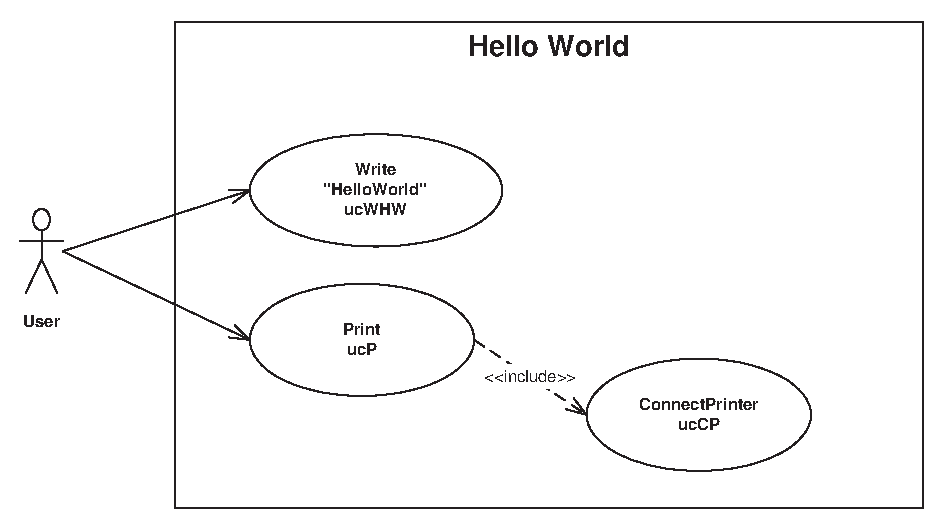
\includegraphics{eps/dsnHelloWorld.eps}}
\caption{\label{Figure::dsnHelloWolrd} Sample EPS image.}
\end{figure}
\end{verbatim}

\noindent
If using Overleaf, then you include a PNG or a JPG file as shown next:

\begin{verbatim}
\begin{figure}
\centering
\scalebox{0.8}{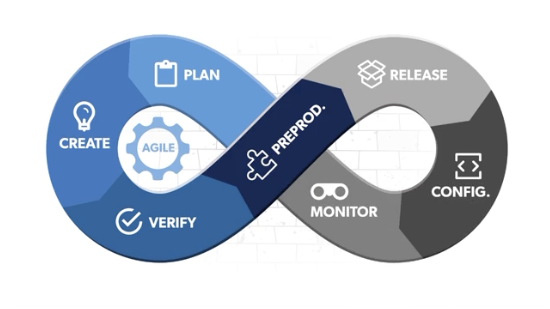
\includegraphics{png/stvAgileProcess.png}}
\caption{\label{Figure::stvAgile} PNG Image included.}
\end{figure}
\end{verbatim}

%\begin{figure}
%\centering
%\scalebox{0.8}{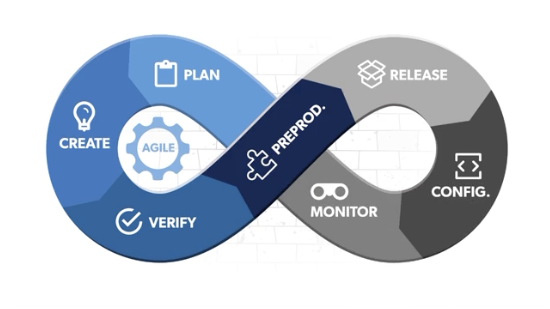
\includegraphics{png/stvAgileProcess.png}}
%\caption{\label{Figure::stvAgileProcess} PNG Image included.}
%\end{figure}

If compiling on Windows, as LaTeX-to-PDF (and not LaTeX-to-PS-to-PDF), 
you need to comment out the pdfmark package from itManual.tex:

\begin{verbatim}
%\usepackage[pdfmark, 
%breaklinks=true, 
%colorlinks=true,
%citecolor=blue,
%linkcolor=blue,
%menucolor=black,
%pagecolor=black,
%urlcolor=blue
%]{hyperref} % links in pdf
\end{verbatim}

\section{Compiling EPS files with PSFrag on Overleaf}

In the header file un-comment the following lines. (Viewable only in the .tex code, not in PDF):

	%\usepackage{graphicx} 
	%\usepackage[process=all]{pstool}
	%\usepackage[ 
	%breaklinks=true, 
	%colorlinks=true,
	%citecolor=blue,
	%linkcolor=blue,
	%menucolor=black,
	%urlcolor=blue
	%]{hyperref}
	%%%%%% 
	%%% NOTE IF LOADING hyperref PACKAGE
	%%% These lines are required ≥TL2020 due to 
	%%% incompatibility between hyperref and preview
	%%% (See https://github.com/latex3/hyperref/issues/166#issuecomment-760157370)
	%\makeatletter
	%\providecommand\HyPL@Entry[1]{}
	%\AddToHook{env/document/begin}{%
	%\@ifpackageloaded{preview}{
	%\ifPreview
		%\let\Hy@FirstPageHook\relax
		%\let\Hy@EveryPageAnchor\relax
	%\fi}{}}
	%\makeatother
	%\end{verbatim}
	%
	%\noindent
	%Then when using the image, use this syntax:
	%\begin{verbatim}
	%\begin{figure}
	%\centering
	%\psfragfig[width=1.0\linewidth]{<path to figure>}{
    %\psfrag{P0 }{\hspace{-0.5in} Test $\sum_0^N$ }
	%}
	%\caption{\label{<label name>} <Caption name>.}
	%\end{figure}

Note that with psfrag used this way, we cannot include references in the psfrag command.  
We can only replace text and use mathematical formulas.

Here is an example glossary term for \gls{should}.
\newpage
\thispagestyle{empty}
\begin{center}
    {\Large\bfseries DevOps - Group 14 Assignments}\\
    \vspace{0.5cm}
    Andre Santiago-Neyra, Badri Narayanan Rajendran\\
    Stevens.edu
\end{center}

\vspace{1cm}

This document provides the group assignments completed by Group 14 for the DevOps course. The following table (Table \ref{Table::UpdateHistory}) should be updated by authors whenever major changes are made to the document or new assignments are added. Add updates to the top of the table. Most recent changes to the document should be seen first and the oldest last.

\vspace{1cm}

\begin{longtable}{|l||p{13.5cm}|}
\caption{Document Update History \label{Table::UpdateHistory}}\\
\hline
\textbf{Date} & \textbf{Updates} \\
\hline 
\endhead
10/27/2025 & Andre, Badri:
\begin{itemize}[topsep=0pt,itemsep=0pt,parsep=0pt,partopsep=0pt,leftmargin=12pt]
\item Assignment 8: Setting up Prometheus & Grafana Dashboards and Node Exporter in DigitalOcean (Chapter \ref{chap:prometheusAndGrafana}).
\end{itemize}
\\ \hline
10/20/2025 & Andre, Badri:
\begin{itemize}[topsep=0pt,itemsep=0pt,parsep=0pt,partopsep=0pt,leftmargin=12pt]
\item Assignment 6: Overleaf CI with GitHub Actions (Chapter \ref{chap:overleafCI}).
\end{itemize}
\\ \hline
10/20/2025 & Andre, Badri:
\begin{itemize}[topsep=0pt,itemsep=0pt,parsep=0pt,partopsep=0pt,leftmargin=12pt]
\item Assignment 5: Overleaf deployment and verification (Chapter \ref{chap:overleafDeployment}).
\end{itemize}
\\ \hline
10/05/2025 & Andre:
\begin{itemize}[topsep=0pt,itemsep=0pt,parsep=0pt,partopsep=0pt,leftmargin=12pt]
\item Assignment 4: Bugzilla and Overleaf Dockers on Digital Ocean (Chapter \ref{chap:digitalocean}).
\end{itemize} 
\\ \hline
10/03/2025 & Andre, Badri:
\begin{itemize}[topsep=0pt,itemsep=0pt,parsep=0pt,partopsep=0pt,leftmargin=12pt]
\item Assignment 3: Docker on AWS created (Chapter \ref{chap:aws}).
\end{itemize} 
\\ \hline
09/24/2025 & Andre:
\begin{itemize}[topsep=0pt,itemsep=0pt,parsep=0pt,partopsep=0pt,leftmargin=12pt]
\item Assignment 2: Project Proposal created (Chapter \ref{chap:proposal}).
\end{itemize} 
\\ \hline
09/17/2025 & Badri:
\begin{itemize}[topsep=0pt,itemsep=0pt,parsep=0pt,partopsep=0pt,leftmargin=12pt]
\item Assignment 1: Linux Commands created (Chapter \ref{chap:linux}).
\end{itemize} 
\\ \hline
09/12/2025 & Andre, Badri, Nozanin:
\begin{itemize}[topsep=0pt,itemsep=0pt,parsep=0pt,partopsep=0pt,leftmargin=12pt]
\item Initial document creation with template structure.
\end{itemize}
\\ \hline
\end{longtable}
\section*{Passwords and Service Hints}
\addcontentsline{toc}{chapter}{Passwords and Service Hints}

This page contains password hints for various services used throughout the assignments. These hints are for reference only and should be updated as credentials change.

\vspace{1cm}

\begin{table}[h]
\centering
\begin{tabular}{|p{4cm}|p{9cm}|}
\hline
\textbf{Service} & \textbf{Password Hint} \\
\hline
Bugzilla Admin & Default password set during deployment (check deployment notes) \\
\hline
MariaDB Root & Password specified in docker-compose environment variables \\
\hline
MariaDB Bugzilla User & Password specified in docker-compose environment variables \\
\hline
Overleaf Admin & Created via command line during setup \\
\hline
DigitalOcean Droplet & SSH key authentication (root user) \\
\hline
AWS Account & SSO credentials via Stevens portal \\
\hline
GitHub & Personal access token for repository access \\
\hline
Docker Hub & Optional - for private image repositories \\
\hline
\end{tabular}
\caption{Service Password Hints}
\label{tab:passwords}
\end{table}

\vspace{1cm}
\chapter{Hosts}

Hosts for my development environment:

\begin{longtable}{p{0.25\textwidth} p{0.25\textwidth} p{0.2\textwidth} p{0.25\textwidth}}
\toprule
\textbf{Hostname} & \textbf{Notes} \\
\midrule
\endfirsthead
\toprule
\textbf{Hostname} & \textbf{Notes} \\
\midrule
\endhead

AWS Elastic Example & Notes here \\

\bottomrule
\end{longtable}

\chapter{Kanban Setup}

This project uses a Kanban board to manage tasks. I set it up using Jira. 

\section*{Steps I followed}
\begin{enumerate}
  \item Created a new Kanban project named ``DevOpsConfiguration''.
  \item Added columns: Backlog, To Do, In Progress, Code Review, Done.
\end{enumerate}

\section*{How I will use it}
\begin{itemize}
  \item Move tasks from To Do → In Progress → Code Review → Done.
  \item Enforce code review before moving to Done.
  \item Use labels to prioritize work.
\end{itemize}

\begin{figure}[h]
\centering
\includegraphics[width=0.9\textwidth]{png/stvagileProcess.png}
\caption{Kanban board example.}
\end{figure}

\chapter{Docker}

\section{Overview}
This chapter documents the installation of Docker on Ubuntu and the successful deployment of two containerized web applications as required for the assignment.

\section{Docker Installation on Ubuntu}
Docker was installed on Ubuntu using the following commands, I had it previously installed so I just verified the installation:

\begin{minted}{bash}
docker --version
docker run hello-world
\end{minted}

\section{First Container: Hello World Web Server}
Created a simple Node.js HTTP server following the assignment instructions. The project structure included \texttt{server.js}, \texttt{package.json}, and \texttt{Dockerfile}.

\subsection{Build and Execution}
\begin{minted}{bash}
docker build -t hello-node .
docker run -p 5050:3000 hello-node
\end{minted}

The application was successfully deployed and accessible at \texttt{http://localhost:5050}.

\begin{figure}[H]
    \centering
    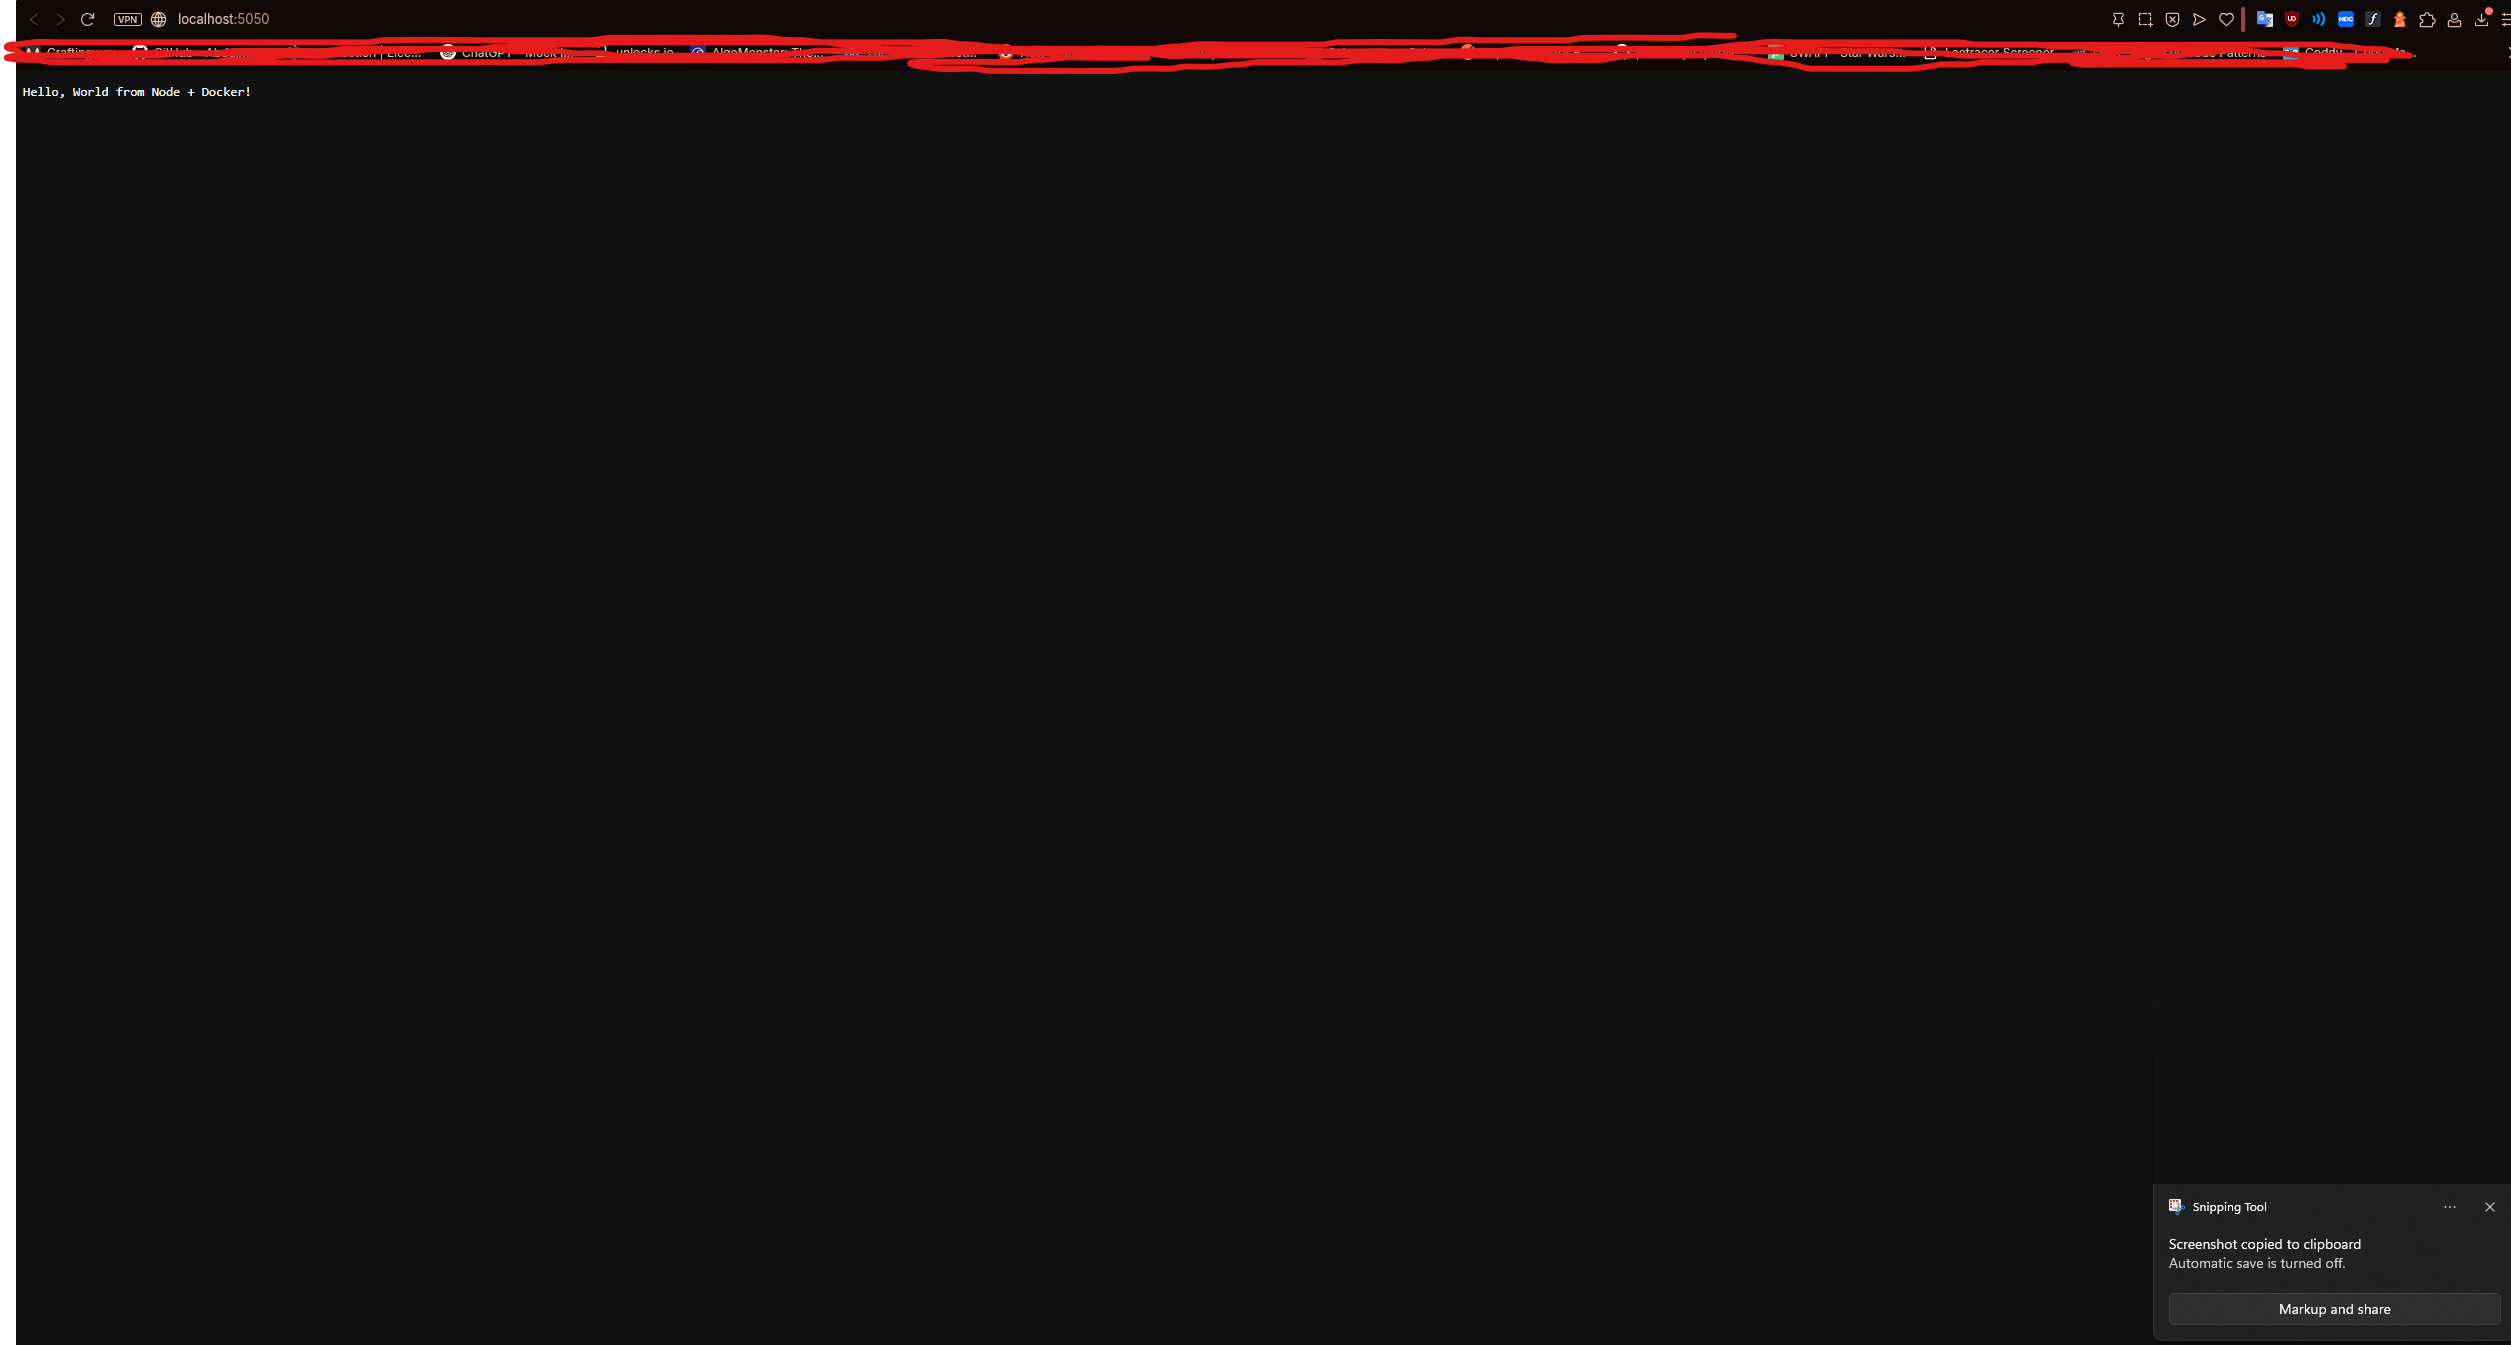
\includegraphics[width=0.8\textwidth]{png/Screenshot 2025-09-23 192048.png}
    \caption{Hello World Node.js application running in Docker container}
    \label{fig:hello-world}
\end{figure}

\section{Second Container: Color Buttons Website}
Created an Express.js web application with interactive color-changing functionality following the assignment specifications.

\subsection{Build and Execution}
\begin{minted}{bash}
docker build -t color-buttons-app .
docker run -p 8080:3000 color-buttons-app
\end{minted}

The application was successfully deployed and accessible at \texttt{http://localhost:8080}.

\begin{figure}[H]
    \centering
    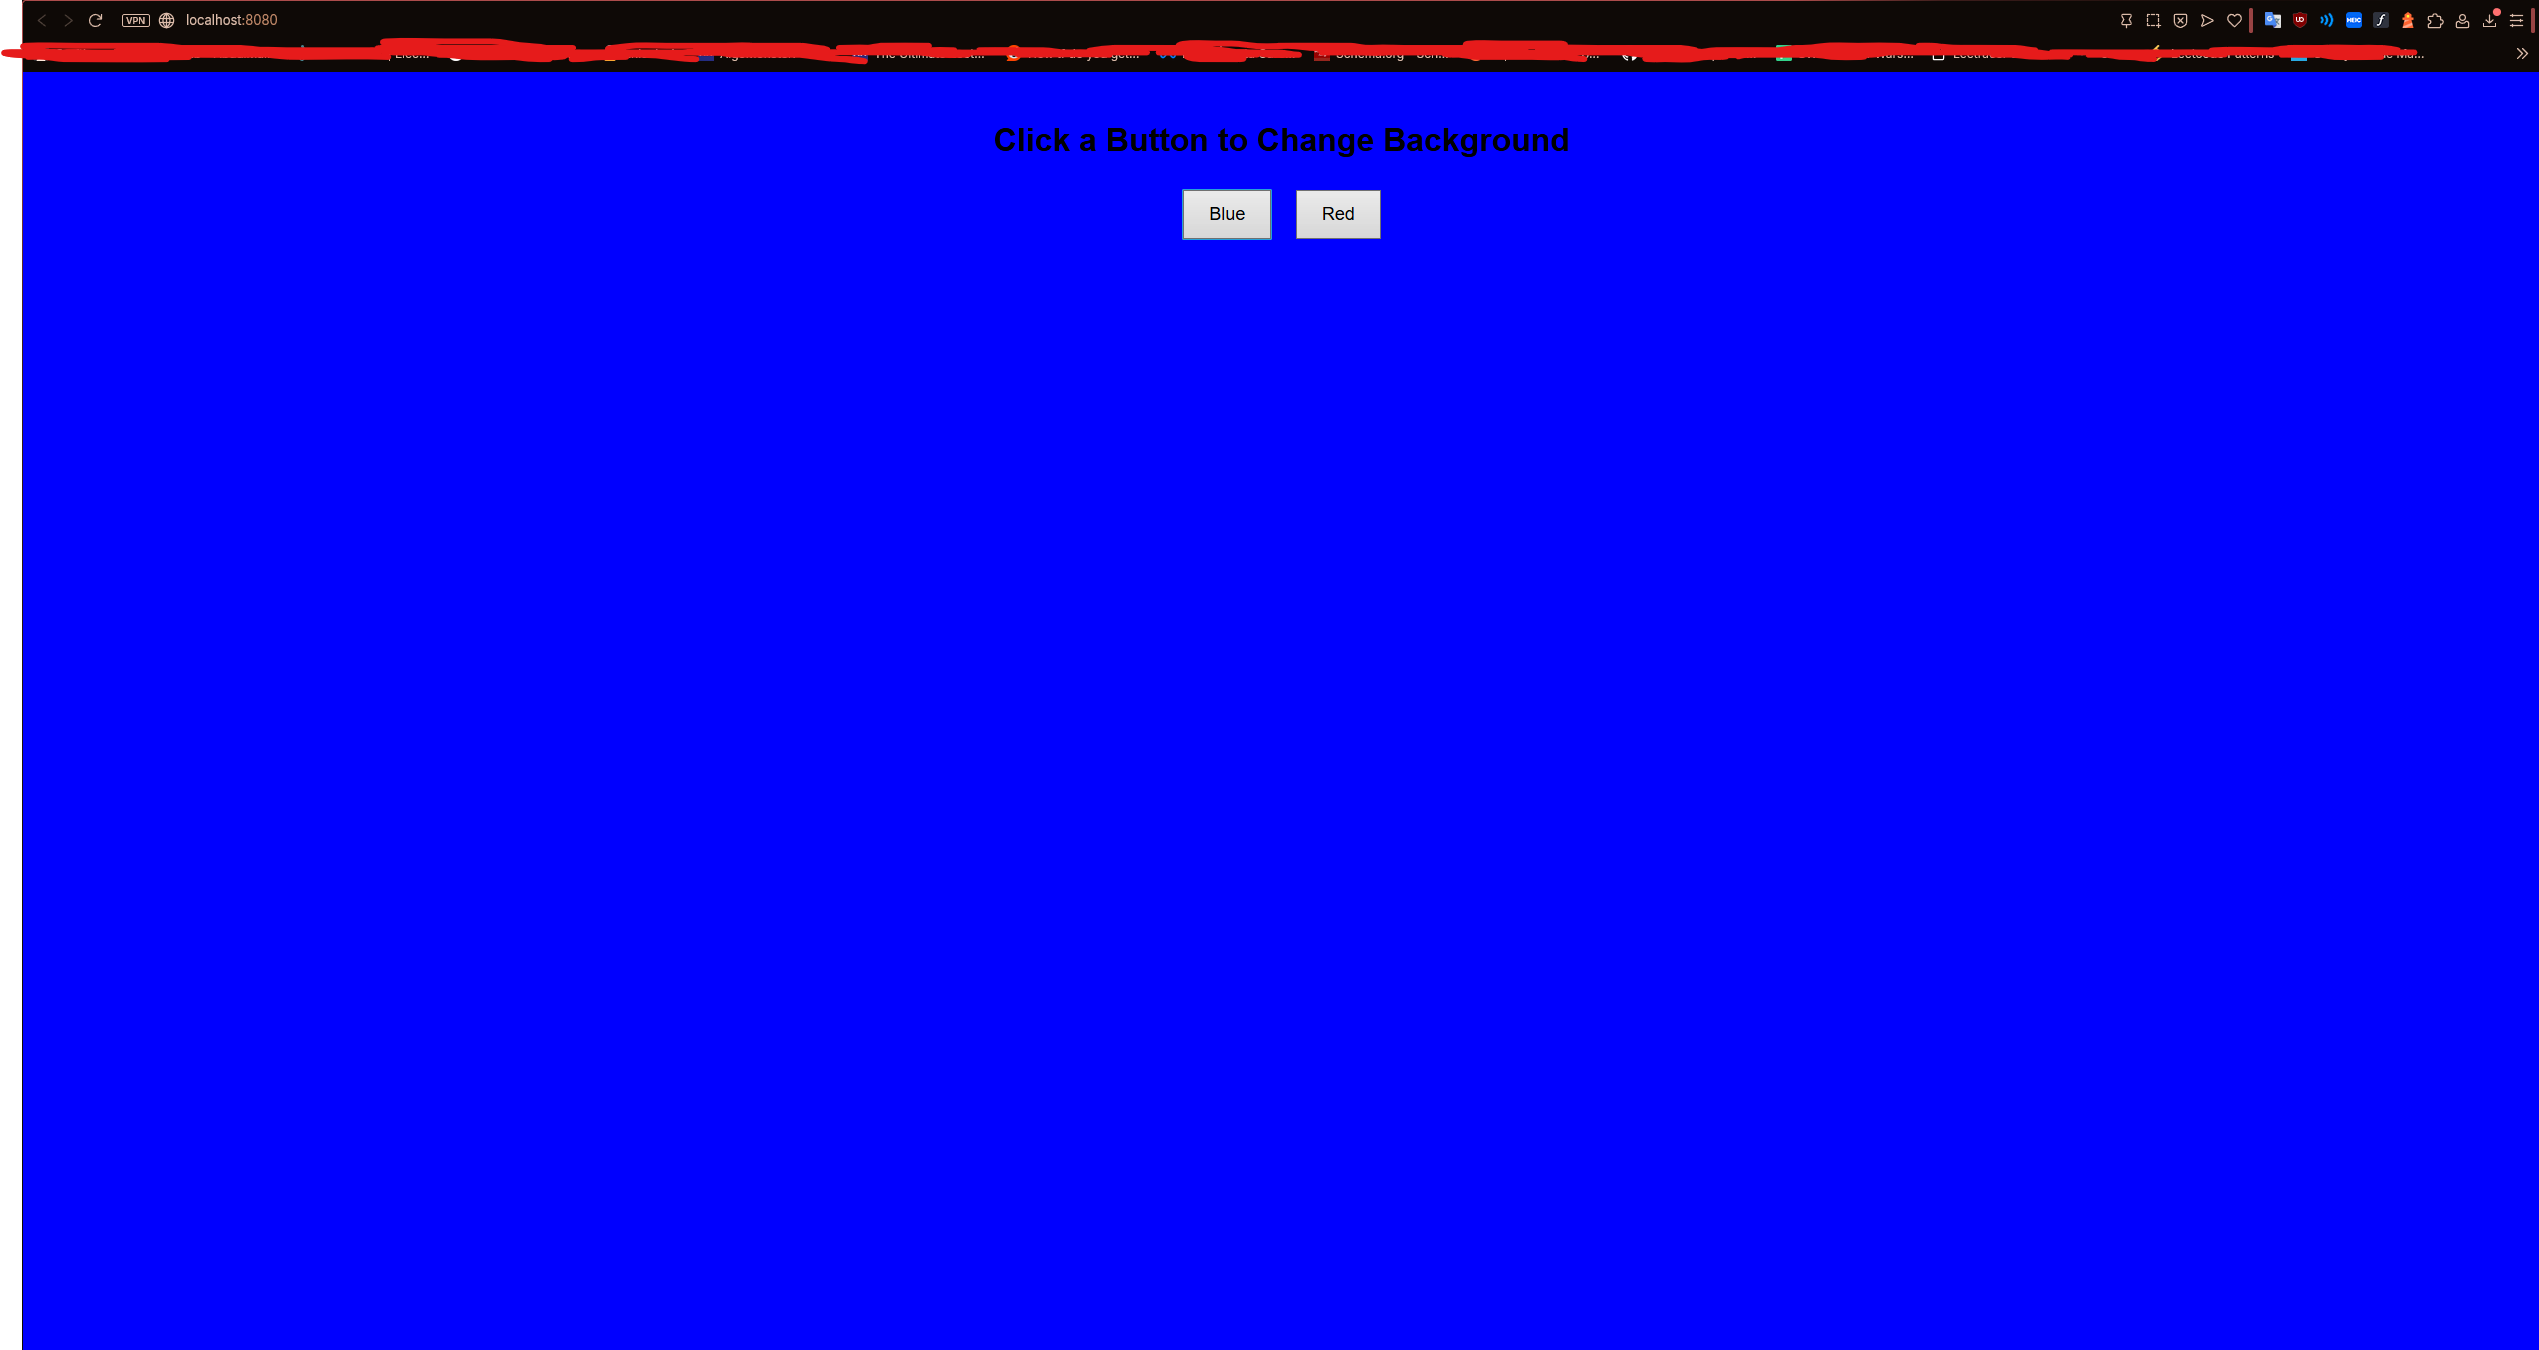
\includegraphics[width=0.8\textwidth]{png/Screenshot 2025-09-23 193125.png}
    \caption{Color Buttons application demonstrating background color change functionality}
    \label{fig:color-buttons}
\end{figure}

\section{Conclusion}
Both Docker containers were successfully created, built, and executed on Ubuntu. The containers ran as expected, serving web content on the mapped ports and demonstrating proper containerization of Node.js applications.
% Chapter 2 - Assignment 2
\chapter{Project Proposal -- Group 14}
\label{chap:proposal}

\section{Project Title}
Automated Blog Deployment Pipeline\index{deployment pipeline}

\section{Project Description}
This project will develop a simple, containerized blog application and automate its build, test, and deployment processes using two \gls{cicd} tools: Jenkins\index{Jenkins} and Github Actions\index{Github Actions}. The application will be hosted on AWS EC2\index{AWS EC2} using Docker\index{Docker}. An operational dashboard, built with monitoring tools, like Grafana, Datadog or Dynatrace, for effectively monitoring of application health and logs.

\section{Simple Tasks}
\begin{itemize}
\item Develop the blog app using Node.js or Python
\item Containerize the app using Docker
\item Integrate source control with GitHub
\item Setup CI/CD with Jenkins and Github Actions for code build, test, and deploy
\item Host on AWS using Docker and ECS
\item Design a dashboard for build and deployment status
\end{itemize}

\section{DevSecOps Tools}
\begin{itemize}
\item Programming Language: Python or Node.js
\item Back-End Framework: Flask or Express
\item Database: PostgreSQL or MongoDB
\item Source Control: GitHub
\item CI/CD: Jenkins, Github Actions
\item Deployment: Docker, AWS EC2, ECS
\item Monitoring: Grafana or Datadog or Dynatrace or similar monitoring tool
\end{itemize}


\appendix
\chapter{Appendix \\
\small{\textit{-- Author Name}}
\index{appendix} 
\index{Chapter!Appendix}
\label{Chapter::Appendix}}

% makeglossaries dsnManual -- from command prompt.
\clearpage
%\printglossaries


\printnoidxglossaries

\bibliography{bibfile}
%\bibliographystyle{unsrt}
\bibliographystyle{IEEEtran}

\printindex
%\input{dsnManual.idx}
\end{document}
